\bta{2007}






\section{Use of English}

\noindent
\textbf{Directions:}\\
Read the following text. Choose the best word (s) for each numbered blank and mark A, B, C or D on ANSWER SHEET 1. (10 points)



\TiGanSpace


By 1830 the former Spanish and Portuguese colonies had become
independent nations. The roughly 20 million \cloze of these
nations looked \cloze to the future. Born in the crisis of the
old regime and Iberian colonialism, many of the leaders of
independence \cloze the ideals of representative government,
careers \cloze to talent, freedom of commerce and trade,
the \cloze to private property, and a belief in the individual as
the basis of society. \cloze there was a belief that the new
nations should be sovereign and independent states, large enough to be
economically viable and integrated by a \cloze set of laws.

On the issue of \cloze of religion and the position of the
Church, \cloze , there was less agreement \cloze the
leadership. Roman Catholicism had been the state religion and the only
one \cloze by the Spanish crown. \cloze most leaders
sought to maintain Catholicism \cloze the official religion of
the new states, some sought to end the \cloze of other faiths.
The defense of the Church became a rallying \cloze for the
conservative forces.

The ideals of the early leaders of independence were often egalitarian,
valuing equality of everything. Bolivar had received aid from Haiti and
had \cloze in return to abolish slavery in the areas he
liberated. By 1854 slavery had been abolished everywhere except
Spain's \cloze colonies. Early promises to end Indian tribute
and taxes on people of mixed origin came much \cloze because the
new nations still needed the revenue such policies \cloze.
Egalitarian sentiments were often tempered by fears that the mass of the
population was \cloze self-rule and democracy.


\newpage

\begin{enumerate}
	%\renewcommand{\labelenumi}{\arabic{enumi}.}
	% A(\Alph) a(\alph) I(\Roman) i(\roman) 1(\arabic)
	%设定全局标号series=example	%引用全局变量resume=example
	%[topsep=-0.3em,parsep=-0.3em,itemsep=-0.3em,partopsep=-0.3em]
	%可使用leftmargin调整列表环境左边的空白长度 [leftmargin=0em]
	\item
\fourchoices
{natives}
{inhabitants}
{peoples}
{individuals}




\item

\fourchoices
{confusedly}
{cheerfully}
{worriedly}
{hopefully}



\item


\fourchoices
{shared}
{forgot}
{attained}
{rejected}




\item


\fourchoices
{related}
{close}
{open}
{devoted}




\item


\fourchoices
{access}
{succession}
{right}
{return}




\item

\fourchoices
{Presumably}
{Incidentally}
{Obviously}
{Generally}


\item


\fourchoices
{unique}
{common}
{particular}
{typical}




\item


\fourchoices
{freedom}
{origin}
{impact}
{reform}




\item


\fourchoices
{therefore}
{however}
{indeed}
{moreover}




\item


\fourchoices
{with}
{about}
{among}
{by}




\item


\fourchoices
{allowed}
{preached}
{granted}
{funded}




\item


\fourchoices
{Since}
{If}
{Unless}
{While}




\item


\fourchoices
{as}
{for}
{under}
{against}




\item

\fourchoices
{spread}
{interference}
{exclusion}
{influence}




\item


\fourchoices
{support}
{cry}
{plea}
{wish}




\item


\fourchoices
{urged}
{intended}
{expected}
{promised}




\item


\fourchoices
{controlling}
{former}
{remaining}
{original}




\item


\fourchoices
{slower}
{faster}
{easier}
{tougher}




\item

\fourchoices
{created}
{produced}
{contributed}
{preferred}



\item

\fourchoices
{puzzled by}
{hostile to}
{pessimistic about}
{unprepared for}

\end{enumerate}

\vfil

\section{Reading Comprehension}


\noindent
\textbf{Part A}\\
\textbf{Directions:}\\
Read the following four texts. Answer the questions below each
text by choosing A, B, C, or D. . Mark your answers on ANSWER SHEET 1. (40 points)

\newpage
\subsection{Text 1}


If you were to examine the birth certificates of every soccer player in
2006's World Cup tournament, you would most likely find a noteworthy
quirk: elite soccer players are more likely to have been born in the
earlier months of the year than in the late months. If you then examined
the European national youth teams that feed the World Cup and
professional ranks, you would find this strange phenomenon to be ever
more pronounced.

What might account for this strange phenomenon? Here are a few guesses:
a) certain astrological signs confer superior soccer skills; b)
winter-born babies tend to have higher oxygen capacity, which increases
soccer stamina; c) soccer-mad parents are more likely to conceive
children in springtime, at the annual peak of soccer \uline{mania};
d) none of the above.

Anders Ericsson, a 58-year-old psychology professor at Florida State
University, says he believes strongly in ``none of the above.'' Ericsson
grew up in Sweden, and studied nuclear engineering until he realized he
would have more opportunity to conduct his own research if he switched
to psychology. His first experiment, nearly 30 years ago, involved
memory: training a person to hear and then repeat a random series of
numbers. ``With the first subject, after about 20 hours of training, his
digit span had risen from 7 to 20,'' Ericsson recalls. ``He kept
improving, and after about 200 hours of training he had risen to over 80
numbers.''

This success, coupled with later research showing that memory itself is
not genetically determined, led Ericsson to conclude that the act of
memorizing is more of a cognitive exercise than an intuitive one. In
other words, whatever inborn differences two people may exhibit in their
abilities to memorize, those differences are swamped by how well each
person ``encodes'' the information. And the best way to learn how to
encode information meaningfully, Ericsson determined, was a process
known as deliberate practice. Deliberate practice entails more than
simply repeating a task. Rather, it involves setting specific goals,
obtaining immediate feedback and concentrating as much on technique as
on outcome.

Ericsson and his colleagues have thus taken to studying expert
performers in a wide range of pursuits, including soccer. They gather
all the data they can, not just performance statistics and biographical
details but also the results of their own laboratory experiments with
high achievers. Their work makes a rather startling assertion: the trait
we commonly call talent is highly overrated. Or, put another way, expert
performers---whether in memory or surgery, ballet or computer
programming---are nearly always made, not born.


\begin{enumerate}[resume]
	%\renewcommand{\labelenumi}{\arabic{enumi}.}
	% A(\Alph) a(\alph) I(\Roman) i(\roman) 1(\arabic)
	%设定全局标号series=example	%引用全局变量resume=example
	%[topsep=-0.3em,parsep=-0.3em,itemsep=-0.3em,partopsep=-0.3em]
	%可使用leftmargin调整列表环境左边的空白长度 [leftmargin=0em]
	\item
 The birthday phenomenon found among soccer players is
mentioned to \lineread.


\fourchoices
{stress the importance of professional training.}
{spotlight the soccer superstars at the World Cup.}
{introduce the topic of what makes expert performance.}
{explain why some soccer teams play better than others.}


\item
The word ``mania'' (Line 4, Paragraph 2) most probably
means \lineread.



\fourchoices
{fun}
{craze}
{hysteria}
{excitement}




\item
According to Ericsson, good memory \lineread.


\fourchoices
{depends on meaningful processing of information}
{results from intuitive rather than cognitive exercises}
{is determined by genetic rather than psychological factors}
{requires immediate feedback and a high degree of concentration}



\item
Ericsson and his colleagues believe that \lineread.


\fourchoices
{talent is a dominating factor for professional success}
{biographical data provide the key to excellent performance}
{the role of talent tends to be overlooked}
{high achievers owe their success mostly to nurture}



\item
Which of the following proverbs is closest to the message
the text tries to convey?


\fourchoices
{``Faith will move mountains.''}
{``One reaps what one sows.''}
{``Practice makes perfect.''}
{``Like father, like son.''}


\end{enumerate}



\newpage
\subsection{Text 2}


For the past several years, the Sunday newspaper
supplement \emph{Parade} has featured a column called ``Ask Marilyn.''
People are invited to query Marilyn vos Savant, who at age 10 had tested
at a mental level of someone about 23 years old; that gave her an IQ of
228---the highest score ever recorded. IQ tests ask you to complete
verbal and visual analogies, to envision paper after it has been folded
and cut, and to deduce numerical sequences, among other similar tasks.
So it is a bit confusing when vos Savant fields such queries from the
average Joe (whose IQ is 100) as, What's the difference between love and
fondness? Or what is the nature of luck and coincidence? It's not
obvious how the capacity to visualize objects and to figure out
numerical patterns suits one to answer questions that have eluded some
of the best poets and philosophers.

Clearly, intelligence encompasses more than a score on a test. Just what
does it mean to be smart? How much of intelligence can be specified, and
how much can we learn about it from neurology, genetics, computer
science and other fields?

The defining term of intelligence in humans still seems to be the IQ
score, even though IQ tests are not given as often as they used to be.
The test comes primarily in two forms: the Stanford-Binet Intelligence
Scale and the Wechsler Intelligence Scales (both come in adult and
children's version). Generally costing several hundred dollars, they are
usually given only by psychologists, although variations of them
populate bookstores and the World Wide Web. Superhigh scores like vos
Savant's are no longer possible, because scoring is now based on a
statistical population distribution among age peers, rather than simply
dividing the mental age by the chronological age and multiplying by 100.
Other standardized tests, such as the Scholastic Assessment Test (SAT)
and the Graduate Record Exam (GRE), capture the main aspects of IQ
tests.

Such standardized tests may not assess all the important elements
necessary to succeed in school and in life, argues Robert J. Sternberg.
In his article ``How Intelligent Is Intelligence Testing?'', Sternberg
notes that traditional tests best assess analytical and verbal skills
but fail to measure creativity and practical knowledge, components also
critical to problem solving and life success. Moreover, IQ tests do not
necessarily predict so well once populations or situations change.
Research has found that IQ predicted leadership skills when the tests
were given under low-stress conditions, but under high-stress
conditions, IQ was negatively correlated with leadership---that is, it
predicted the opposite. Anyone who has toiled through SAT will testify
that test-taking skill also matters, whether it's knowing when to guess
or what questions to skip.

\begin{enumerate}[resume]
	%\renewcommand{\labelenumi}{\arabic{enumi}.}
	% A(\Alph) a(\alph) I(\Roman) i(\roman) 1(\arabic)
	%设定全局标号series=example	%引用全局变量resume=example
	%[topsep=-0.3em,parsep=-0.3em,itemsep=-0.3em,partopsep=-0.3em]
	%可使用leftmargin调整列表环境左边的空白长度 [leftmargin=0em]
	\item
Which of the following may be required in an intelligence
test?


\fourchoices
{Answering philosophical questions.}
{Folding or cutting paper into different shapes.}
{Telling the differences between certain concepts.}
{Choosing words or graphs similar to the given ones.}



\item
What can be inferred about intelligence testing from
Paragraph 3?


\fourchoices
{People no longer use IQ scores as an indicator of intelligence.}
{More versions of IQ tests are now available on the Internet.}
{The test contents and formats for adults and children may be different.}
{Scientists have defined the important elements of human intelligence.}



\item
People nowadays can no longer achieve IQ scores as high as
vos Savant's because  \lineread.


\fourchoices
{the scores are obtained through different computational procedures}
{creativity rather than analytical skills is emphasized now}
{vos Savant's case is an extreme one that will not repeat}
{the defining characteristic of IQ tests has changed}



\item
We can conclude from the last paragraph that \lineread.


\fourchoices
{test scores may not be reliable indicators of one's ability}
{IQ scores and SAT results are highly correlated}
{testing involves a lot of guesswork}
{traditional tests are out of date}


\item
What is the author's attitude towards IQ tests?


\fourchoices
{Supportive.}
{Skeptical.}
{Impartial.}
{Biased.}


\end{enumerate}



\newpage
\subsection{Text 3}


During the past generation, the American middle-class family that once
could count on hard work and fair play to keep itself financially secure
has been transformed by economic risk and new realities. Now a pink slip,
a bad diagnosis, or a disappearing spouse can reduce a family from
solidly middle class to newly poor in a few months.

In just one generation, millions of mothers have gone to
work, transforming basic family economics. Scholars, policymakers, and
critics of all stripes have debated the social implications of these
changes, but few have looked at the side effect: family risk has risen
as well. Today's families have budgeted to the limits of theirs new
two-paycheck status. As a result, they have lost the parachute they once
had in times of financial setback---a back-up earner (usually Mom) who
could go into the workforce if the primary earner got laid off or fell
sick. This ``added-worker effect'' could support the safety net offered
by unemployment insurance or disability insurance to help families
weather bad times. But today, a disruption to family fortunes can no
longer be made up with extra income from an otherwise-stay-at-home
partner.

During the same period, families have been asked to absorb much more
risk in their retirement income. Steelworkers, airline employees, and
now those in the auto industry are joining millions of families who must
worry about interest rates, stock market fluctuation, and the harsh
reality that they may outlive their retirement money. For much of the
past year, President Bush campaigned to move Social Security to a
savings-account model, with retirees trading much or all of their
guaranteed payments for payments depending on investment returns. For
younger families, the picture is not any better. Both the absolute cost
of healthcare and the share of it borne by families have risen---and
newly fashionable health-savings plans are spreading from legislative
halls to Wal-Mart workers, with much higher deductibles and a large new
dose of investment risk for families' future healthcare. Even
demographics are working against the middle class family, as the odds of
having a weak elderly parent---and all the attendant need for physical
and financial assistance---have jumped eightfold in just one generation.

From the middle-class family perspective, much of this, understandably,
looks far less like an opportunity to exercise more financial
responsibility, and a good deal more like a frightening acceleration of
the wholesale shift of financial risk onto their already overburdened
shoulders. The financial fallout has begun, and the political fallout
may not be far behind.

\begin{enumerate}[resume]
	%\renewcommand{\labelenumi}{\arabic{enumi}.}
	% A(\Alph) a(\alph) I(\Roman) i(\roman) 1(\arabic)
	%设定全局标号series=example	%引用全局变量resume=example
	%[topsep=-0.3em,parsep=-0.3em,itemsep=-0.3em,partopsep=-0.3em]
	%可使用leftmargin调整列表环境左边的空白长度 [leftmargin=0em]
	\item
Today's double-income families are at greater financial risk
in that \lineread.


\fourchoices
{the safety net they used to enjoy has disappeared}
{their chances of being laid off have greatly increased}
{they are more vulnerable to changes in family economics}
{they are deprived of unemployment or disability insurance}



\item
As a result of President Bush's reform, retired people may
have \lineread.


\fourchoices
{a higher sense of security}
{less secured payments}
{less chance to invest}
{a guaranteed future}




\item
According to the author, health-savings plans will \lineread.


\fourchoices
{help reduce the cost of healthcare}
{popularize among the middle class}
{compensate for the reduced pensions}
{increase the families' investment risk}



\item
 It can be inferred from the last paragraph that \lineread.


\fourchoices
{financial risks tend to outweigh political risks}
{the middle class may face greater political challenges}
{financial problems may bring about political problems}
{financial responsibility is an indicator of political status}


\item
Which of the following is the best title for this text?


\fourchoices
{The Middle Class on the Alert}
{The Middle Class on the Cliff}
{The Middle Class in Conflict}
{The Middle Class in Ruins}


\end{enumerate}


\newpage
\subsection{Text 4}


\uline{It never rains but it pours}. Just as bosses and boards have finally
sorted out their worst accounting and compliance troubles, and improved
their feeble corporation governance, a new problem threatens to earn
them---especially in America---the sort of nasty headlines that
inevitably lead to heads rolling in the executive suite: data
insecurity. Left, until now, to odd, low-level IT staff to put right,
and seen as a concern only of data-rich industries such as banking,
telecoms and air travel, information protection is now high on the
boss's agenda in businesses of every variety.

Several massive leakages of customer and employee data this year---from
organizations as diverse as Time Warner, the American defense contractor
Science Applications International Corp and even the University of
California, Berkeley---have left managers hurriedly peering into their
intricate IT systems and business processes in search of potential
vulnerabilities.

``Data is becoming an asset which needs to be guarded as much as any
other asset,'' says Haim Mendelson of Stanford University's business
school. ``The ability to guard customer data is the key to market value,
which the board is responsible for on behalf of shareholders.'' Indeed,
just as there is the concept of Generally Accepted Accounting Principles
(GAAP), perhaps it is time for GASP, Generally Accepted Security
Practices, suggested Eli Noam of New York's Columbia Business School.
``Setting the proper investment level for security, redundancy, and
recovery is a management issue, not a technical one,'' he says.

The mystery is that this should come as a surprise to any boss. Surely
it should be obvious to the dimmest executive that trust, that most
valuable of economic assets, is easily destroyed and hugely expensive to
restore---and that few things are more likely to destroy trust than a
company letting sensitive personal data get into the wrong hands.

The current state of affairs may have been encouraged---though not
justified---by the lack of legal penalty (in America, but not Europe)
for data leakage. Until California recently passed a law, American firms
did not have to tell anyone, even the victim, when data went astray.
That may change fast: lots of proposed data-security legislation is now
doing the rounds in Washington,
D.C. Meanwhile, the theft of information
about some 40 million credit-card accounts in America, disclosed on June
17th, overshadowed a hugely important decision a day
earlier by America's Federal Trade Commission (FTC) that puts corporate
America on notice that regulators will act if firms fail to provide
adequate data security.

\begin{enumerate}[resume]
	%\renewcommand{\labelenumi}{\arabic{enumi}.}
	% A(\Alph) a(\alph) I(\Roman) i(\roman) 1(\arabic)
	%设定全局标号series=example	%引用全局变量resume=example
	%[topsep=-0.3em,parsep=-0.3em,itemsep=-0.3em,partopsep=-0.3em]
	%可使用leftmargin调整列表环境左边的空白长度 [leftmargin=0em]
	\item
The statement ``It never rains but it pours'' is used to
introduce \lineread.


\fourchoices
{the fierce business competition}
{the feeble boss-board relations}
{the threat from news reports}
{the severity of data leakage.}



\item
 According to Paragraph 2, some organizations check their
systems to find out \lineread.


\fourchoices
{whether there is any weak point}
{what sort of data has been stolen}
{who is responsible for the leakage}
{how the potential spies can be located}



\item
In bringing up the concept of GASP the author is making the
point that \lineread.


\fourchoices
{shareholders' interests should be properly attended to}
{information protection should be given due attention}
{businesses should enhance their level of accounting security}
{the market value of customer data should be emphasized}



\item
 According to Paragraph 4, what puzzles the author is that
some bosses fail to \lineread.


\fourchoices
{see the link between trust and data protection}
{perceive the sensitivity of personal data}
{realize the high cost of data restoration}
{appreciate the economic value of trust}



\item
It can be inferred from Paragraph 5 that \lineread.


\fourchoices
{data leakage is more severe in Europe}
{FTC's decision is essential to data security}
{California takes the lead in security legislation}
{legal penalty is a major solution to data leakage}


\end{enumerate}



\newpage

\noindent
\textbf{Part B}\\
\textbf{Directions:}\\
You are going to read a list of headings and a text about what
parents are supposed to do to guide their children into adulthood.
Choose a heading from the list A-G that best fits the meaning of each
numbered part of the text (41-45). The first and last paragraphs of the
text are not numbered. There are two extra headings that you do not need
to use. Mark your answers on ANSWER SHEET 1. (10 points)


\TiGanSpace


\begin{listmatch}
\item 
Set a Good Example for Your Kids


\item 
Build Your Kids' Work Skills


\item 
Place Time Limits on Leisure Activities


\item 
Talk about the Future on a Regular Basis


\item 
Help Kids Develop Coping Strategies


\item 
Help Your Kids Figure Out Who They Are


\item 
 Build Your Kids' Sense of Responsibility
\end{listmatch}



\begin{center}
\textbf{How Can a Parent Help?}
\end{center}


Mothers and fathers can do a lot to ensure a safe landing in early
adulthood for their kids. Even if a job's starting salary seems too
small to satisfy an emerging adult's need for rapid content, the
transition from school to work can be less of a setback if the start-up
adult is ready for the move. Here are a few measures, drawn from my
book \emph{Ready or Not, Here Life Comes}, that parents can take to
prevent what I call ``work-life unreadiness'':


 \begin{tabular}{|c|c|}
 \hline 
41.  &   \hspace{10em}  \\ 
 \hline 
 \end{tabular}



You can start this process when they are 11 or 12. Periodically review
their emerging strengths and weaknesses with them and work together on
any shortcomings, like difficulty in communicating well or
collaborating. Also, identify the kinds of interests they keep coming
back to, as these offer clues to the careers that will fit them best.

 \begin{tabular}{|c|c|}
	\hline 
	42.  &   \hspace{10em}  \\ 
	\hline 
\end{tabular}

Kids need a range of authentic role models---as opposed to members of
their clique, pop stars and vaunted athletes. Have regular dinner-table
discussions about people the family knows and how they got where they
are. Discuss the joys and downsides of your own career and encourage
your kids to form some ideas about their own future. When asked what
they want to do, they should be discouraged from saying ``I have no
idea.'' They can change their minds 200 times, but having only a foggy
view of the future is of little good.

 \begin{tabular}{|c|c|}
	\hline 
	43.  &   \hspace{10em}  \\ 
	\hline 
\end{tabular}

Teachers are responsible for teaching kids how to learn; parents should
be responsible for teaching them how to work. Assign responsibilities
around the house and make sure homework deadlines are met. Encourage
teenagers to take a part-time job. Kids need plenty of practice delaying
gratification and deploying effective organizational skills, such as
managing time and setting priorities.

 \begin{tabular}{|c|c|}
	\hline 
	44.  &   \hspace{10em}  \\ 
	\hline 
\end{tabular}

Playing video games encourages immediate content. And hours of watching
TV shows with canned laughter only teaches kids to process information
in a passive way. At the same time, listening through earphones to the
same monotonous beats for long stretches encourages kids to stay inside
their bubble instead of pursuing other endeavors. All these activities
can prevent the growth of important communication and thinking skills
and make it difficult for kids to develop the kind of sustained
concentration they will need for most jobs.



 \begin{tabular}{|c|c|}
	\hline 
	45.  &   \hspace{10em}  \\ 
	\hline 
\end{tabular}


They should know how to deal with setbacks, stress and feelings of
inadequacy. They should also learn how to solve problems and resolve
conflicts, ways to brainstorm and think critically. Discussions at home
can help kids practice doing these things and help them apply these
skills to everyday life situations.

What about the son or daughter who is grown but seems to be struggling
and wandering aimlessly through early adulthood? Parents still have a
major role to play, but now it is more delicate. They have to be careful
not to come across as disappointed in their child. They should exhibit
strong interest and respect for whatever currently interests their
fledging adult (as naive or ill conceived as it may seem) while becoming
a partner in exploring options for the future. Most of all, these new
adults must feel that they are respected and supported by a family that
appreciates them.

%刷新计数器
\phantom{\linefill.\linefill.\linefill.\linefill.\linefill.}



\noindent
\textbf{Part C}\\
\textbf{Directions:}\\
Read the following text carefully and then translate the
underlined segments into Chinese. Your translation should be written
neatly on \textbf{ANSWER SHEET 2}. (10 points)


The study of law has been recognized for centuries as a basic
intellectual discipline in European universities. However, only in
recent years has it become a feature of undergraduate programs in
Canadian universities. \transnum \uline{Traditionally, legal learning has
been viewed in such institutions as the special preserve of lawyers,
rather than a necessary part of the intellectual equipment of an
educated person.} Happily, the older and more continental view of legal
education is establishing itself in a number of Canadian universities
and some have even begun to offer undergraduate degrees in law.

If the study of law is beginning to establish itself as part and parcel
of a general education, its aims and methods should appeal directly to
journalism educators. Law is a discipline which encourages responsible
judgment. On the one hand, it provides opportunities to analyze such
ideas as justice, democracy and freedom. \transnum \uline{On the other,
it links these concepts to everyday realities in a manner which is
parallel to the links journalists forge on a daily basis as they cover
and comment on the news.} For example, notions of evidence and fact, of
basic rights and public interest are at work in the process of
journalistic judgment and production just as in courts of law.
Sharpening judgment by absorbing and reflecting on law is a desirable
component of a journalist's intellectual preparation for his or her
career.

\transnum \uline{But the idea that the journalist must understand the law
more profoundly than an ordinary citizen rests on an understanding of
the established conventions and special responsibilities of the news
media.} Politics or, more broadly, the functioning of the state, is a
major subject for journalists. The better informed they are about the
way the state works, the better their reporting will be.
\transnum \uline{In fact, it is difficult to see how journalists who do
not have a clear grasp of the basic features of the Canadian
Constitution can do a competent job on political stories.}

Furthermore, the legal system and the events which occur within it are
primary subjects for journalists. While the quality of legal journalism
varies greatly, there is an undue reliance amongst many journalists on
interpretations supplied to them by lawyers. \transnum \uline{While
comment and reaction from lawyers may enhance stories, it is preferable
for journalists to rely on their own notions of significance and make
their own judgments.} These can only come from a well-grounded
understanding of the legal system.




\newpage

\section{Writing}


\noindent
\textbf{Part A}\\
\textbf{51. Directions:}

Write a letter to your university library, making suggestions for
improving its service.

You should write about 100 words on ANSWER SHEET 2.

\textbf{Do not} sign your own name at the end of the letter. Use ``Li
Ming'' instead.

\textbf{Do not} write the address. (10 points)


\vspace{2em}


\noindent
\textbf{Part B}\\
\textbf{52. Directions:}

Write an essay of 160-200 words based on the following drawing. In your
essay, you should
\begin{listwrite}
	\item
 describe the drawing briefly,

\item 
 explain its intended meaning, and then

\item 
 support your view with an example/examples.
\end{listwrite}

You should write neatly on ANSWER SHEET 2. (20 points)

\begin{figure}[h!]
	\centering
	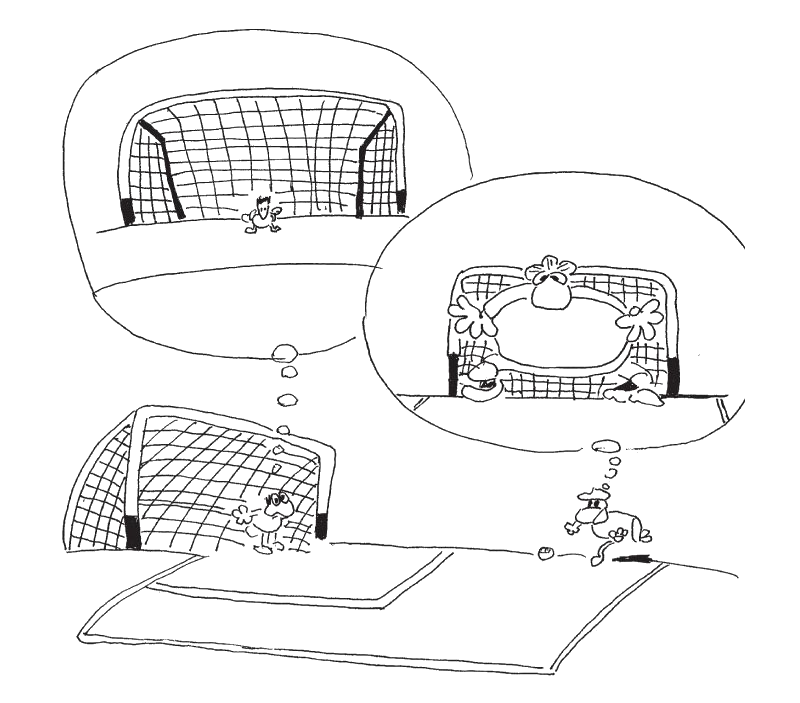
\includegraphics[width=0.56\linewidth]{picture/2007.png}
\end{figure}

